% !TEX program = lualatex
\documentclass[11pt]{article}

% -------- LuaLaTeX : polices et langue --------
\usepackage{fontspec}
\setmainfont{Latin Modern Roman}
\setsansfont{Tex Gyre Heros}
%\renewcommand{\familydefault}{\sfdefault} % force le sans serif par défaut
\usepackage{polyglossia}
\setdefaultlanguage{french}

% -------- Mise en page --------
\usepackage[a4paper,margin=1cm]{geometry}
\usepackage{multicol}
\usepackage{fancyhdr}
\pagestyle{empty}
\usepackage[most]{tcolorbox}

% -------- Mathématiques --------
\usepackage{amsmath,amssymb,mathtools}
% \usepackage{siunitx}
% \sisetup{locale=FR}

\usepackage{enumitem}
\setlist[itemize]{left=0pt}
\setlist[enumerate]{left=0pt, label=\textbf{\arabic*}.}

\usepackage{ProfCollege}
\usepackage{ProfMaquette}

%\usepackage{tabularray}
\usepackage{tabularx}

% -------- Divers --------
\newcommand{\ligne}{{\color{gray!60}\hrulefill}}

\setlength{\parindent}{0pt}

\begin{document}



\begin{Maquette}[IE]{
        Numero = 1, Code={}, Date = Lundi 29 septembre, Theme = Arithmétique / Calcul littéral / Géométrie, Calculatrice = true
    }


    \begin{exercice}
        \begin{enumerate}
            \item \brm{1} Rappelle la définition d’un nombre \emph{premier}. \ligne
            \item[] \ligne
            \item Sans justification, écris :
                  \begin{itemize}
                      \item \brm{.5}la liste de tous les diviseurs du nombre $30$ : \ligne
                      \item \brm{.5}les deux multiples de $9$ compris entre $2120$ et $2140$ : \ligne
                      \item \brm{.5}tous les nombres premiers compris entre $10$ et $30$ : \ligne
                  \end{itemize}
        \end{enumerate}
    \end{exercice}

    \begin{exercice}
        \brm{5}Une collectionneuse compte ses cartes Pokémon afin de les revendre.

        Elle possède $180$ cartes de type «\emph{feu}» et $156$ cartes de type «\emph{terre}».

        \begin{enumerate}[itemsep=1em]
            \item Parmi les trois propositions suivantes, laquelle correspond à la décomposition en produit de facteurs premiers du nombre $180$ ?
                  \begin{center}
                      \renewcommand{\arraystretch}{1.2}
                      \begin{tabular}{|*{3}{c|}}
                          \hline
                          Proposition 1       & Proposition 2             & Proposition 3         \\
                          $2^2\times9\times5$ & $2\times2\times3\times15$ & $2^2\times3^2\times5$ \\
                          \hline
                      \end{tabular}
                  \end{center}
            \item Trouver la décomposition en produit de facteurs premiers du nombre $156$.
            \item Elle veut réaliser des paquets identiques, c'est-à-dire contenant chacun le même nombre de cartes «\emph{terre}»  et le même nombre de cartes «\emph{feu}»  en utlisant toutes les cartes.
                  \begin{enumerate}[label=\textbf{\alph*.}]
                      \item Peut-elle faire $36$ paquets ?
                      \item Quel est le nombre maximum de paquets qu'elle peut réaliser ?
                      \item Combien de cartes de chaque type contient alors chaque paquet ?
                  \end{enumerate}
            \item Elle choisit une carte au hasard parmi toutes ses cartes. On suppose les cartes indiscernables au toucher. Calculer la probabilité que ce soit une carte de type «\emph{terre}».
        \end{enumerate}
    \end{exercice}

    \begin{multicols}{2}
        \begin{exercice}
            \brm{2} Relier proprement chaque expression à son écriture réduite.
            \begin{center}
                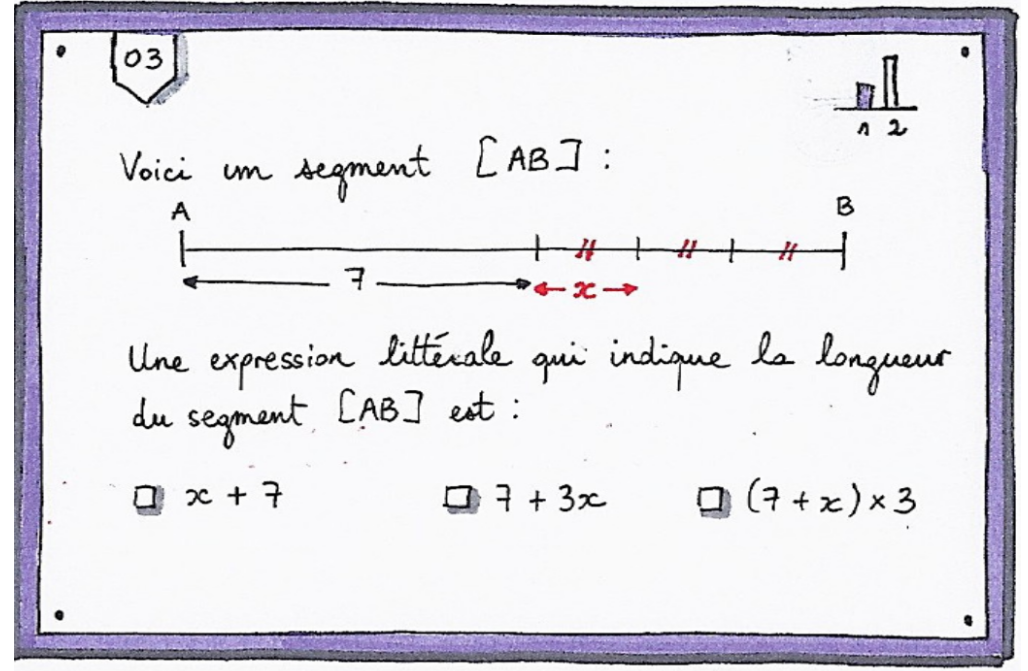
\includegraphics[width=.8\linewidth]{Images/CalculLitteral1.png}
            \end{center}
        \end{exercice}
        \columnbreak
        \begin{exercice}
            \brm{5,5}Recopier et réduire chacune des expressions littérales suivantes. Rédiger en montrant les étapes intermédiaires.
            \begin{itemize}
                \item $\textrm{A}=8 - 2 \times s + s \times 5$
                \item $\textrm{B}=x \times 5 - 3 - x \times 4$
                \item $\textrm{C}= 7a + (-2 + 3a) + 5$
                \item $\textrm{D}= - (- 3b + 2) + 7b$
                \item $\textrm{E}=(5c - 2) + 2c - (8 - 6c)$
            \end{itemize}
        \end{exercice}
    \end{multicols}

    \begin{exercice}
            \emph{Extrait d’un exercice du DNB 2023 − Centres étrangers}
            \begin{center}
                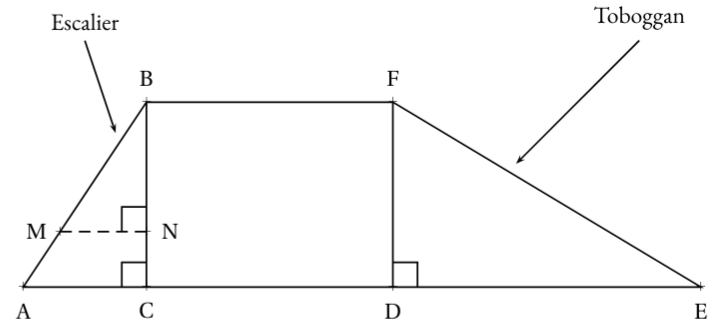
\includegraphics[width=.75\linewidth]{Images/Géométrie1.png}
            \end{center}
            \brm{3} On sait que :
            \begin{center}
                      \renewcommand{\arraystretch}{1.2}
                      \begin{tabular}{|*{4}{c|}}
                          \hline
                      AB = 2,6 m       & AC = 1 m             &  BC = DF = 2,4 m & DE = 4,08 m         \\
                          \hline
                      \end{tabular}
                  \end{center}
 
        Calculer la longueur de la rampe du tobogan EF.
    \end{exercice}
    \begin{exercice}
        \begin{multicols}{2}
            \brm{2} GMK est un triangle tel que :
            \begin{itemize}
                \item le point B appartient au côté [GK]
                \item le point H appartient au côté [GM]
                \item les droites (BH) et (KM) sont parallèles
                \item KM = \Lg{54}, BH = \Lg{45} et GK = \Lg{48}
            \end{itemize}
            \columnbreak
            \begin{center}
                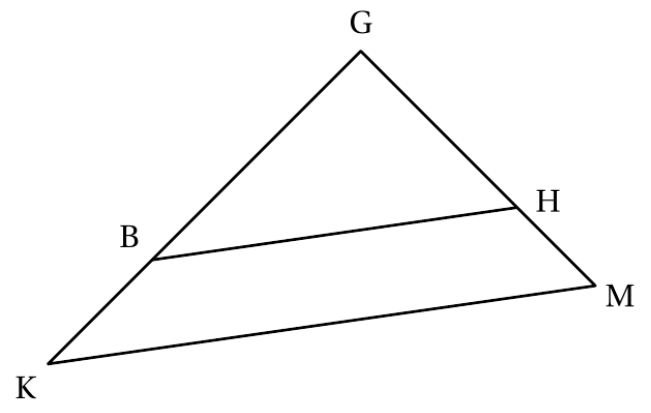
\includegraphics[width=.9\linewidth]{Images/Géométrie2.png}

                \emph{Le dessin n’est pas à l’échelle.}
            \end{center}
            
        \end{multicols}
            \begin{enumerate}
                \item Écrire les trois fractions de Thalès qui sont égales dans cette situation.
                \item Calculer la longueur GB.
        \end{enumerate}
    \end{exercice}
\end{Maquette}


\end{document}